% ============================================================
%  PRESENTATION: AI-Driven Packet Forwarding With PDP
%  Course:       Next Generation Network Infrastructures & Services
%  Author:       Katsimpras Drosos (ais25123)
%  University:   Harokopio University of Athens – DIT
%  Supervisor:   Dr. Liotou Eirini
%  Academic Year: 2025-2026
%
%  Compile with: pdflatex presentation.tex
% ============================================================

\documentclass[8pt, aspectratio=169]{beamer}

% ── Theme ────────────────────────────────────────────────────
\usetheme[progressbar=frametitle]{metropolis}
\usepackage{appendixnumberbeamer}

% ── Core Packages ────────────────────────────────────────────
\usepackage{xcolor}
\usepackage{tcolorbox}
    \tcbuselibrary{skins}
\usepackage{booktabs}
\usepackage{multirow}
\usepackage{comment}
\usepackage{fontawesome5}
\usepackage{array}
\usepackage{pgfplots}
    \usepgfplotslibrary{dateplot}
\usepackage[scale=3]{ccicons}
\usepackage{xspace}
\usepackage{colortbl}
\usepackage{booktabs}
\usepackage{url}
\usepackage{hyperref}
\hypersetup{
  colorlinks=true,
  linkcolor=HUAblue,
  urlcolor=HUAblue,
  citecolor=HUAblue
}

% ── University Colour (HUA) ──────────────────────────────────
%    Primary brand colour used for all headers and UI elements
\definecolor{HUAblue}  {HTML}{005A8C}   % Official HUA blue
\definecolor{HUAdark}  {HTML}{003A5C}   % Darker shade → stat backgrounds
\definecolor{HUAlight} {HTML}{4A90B8}   % Lighter shade → stat numbers
\definecolor{HUApale}  {HTML}{D6EAF4}   % Very light   → card backgrounds
\definecolor{HUAfooter}{HTML}{8EAFC2}   % Muted        → footer text

% ── Semantic Colours (used for content meaning) ──────────────
%    Orange  → problems / bottlenecks
%    Red     → critical issues / limitations
%    Green   → solutions / goals / results
\definecolor{problemorange}{HTML}{E67E22}
\definecolor{problemred}   {HTML}{C0392B}
\definecolor{solutiongreen}{HTML}{27AE60}

% ── Backwards compatibility aliases ─────────────────────────
\definecolor{accent}   {HTML}{4A90B8}   % = HUAlight
\definecolor{accent2}  {HTML}{005A8C}   % = HUAblue
\definecolor{warncolor}{HTML}{E67E22}   % = problemorange
\definecolor{darkbg}   {HTML}{003A5C}   % = HUAdark
\definecolor{cardface} {HTML}{D6EAF4}   % = HUApale

% ── Metropolis Theme Overrides ───────────────────────────────
%    Keep all UI elements in HUA brand colours
\setbeamercolor{palette primary}          {fg=white,    bg=HUAblue}
\setbeamercolor{progress bar}             {fg=HUAblue,  bg=gray!30}
\setbeamercolor{title separator}          {fg=HUAblue}
\setbeamercolor{progress bar in head/foot}{fg=HUAblue,  bg=gray!30}
\setbeamercolor{footline}                 {fg=HUAblue!70}
\setbeamercolor{block title}              {fg=white,    bg=HUAblue}
\setbeamercolor{block body}               {fg=HUAdark,  bg=HUApale}

% ── Footer ───────────────────────────────────────────────────
\setbeamertemplate{frame footer}{HUA -- DIT \textbar{} Katsimpras Drosos}

% ── Stat Box ─────────────────────────────────────────────────
\tcbset{
  statbox/.style={
    enhanced,
    boxrule  = 0pt,
    colback  = HUAblue,    
    colframe = HUAdark,    
    arc      = 4pt,
    left=8pt, right=8pt, top=18pt, bottom=18pt,
    height   = 1.50cm,
    valign   = center,
  },
  problemcard/.style={
    enhanced,
    boxrule  = 0pt,
    colback  = white,    
    colframe = white,
    arc      = 4pt,
    left=8pt, right=6pt, top=5pt, bottom=5pt,
    borderline west={4pt}{0pt}{#1},
  }
}

% ── Subtitle Bar ─────────────────────────────────────────────
%    Usage: \subtitlebar{Your subtitle here}
%    → HUA blue bar below frame title, italic white text
\newcommand{\subtitlebar}[1]{%
  \vspace{-0.10cm}%
  \begin{beamercolorbox}[wd=\textwidth, ht=0.32cm, dp=0.08cm,
                         leftskip=0.25cm]{block title}%
    \color{white}\itshape\fontsize{8}{9}\selectfont #1%
  \end{beamercolorbox}%
  \vspace{0.08cm}%
}

\newcommand{\abbr}[2]{%
  {\color{HUAblue}\bfseries\footnotesize #1} &
  {\footnotesize\color{HUAdark} #2} \\[5pt]
}

% ── Helpers ──────────────────────────────────────────────────
\newcommand{\themename}{\textbf{\textsc{metropolis}}\xspace}

% ── Title Slide Metadata ─────────────────────────────────────
\title{Next Generation Network Infrastructures and Services}
\subtitle{AI-Driven Packet Forwarding With Programmable Data Plane: A Survey}
\author{Katsimpras Drosos (ais25123)}
\institute{%
  Harokopio University of Athens\\
  Department of Informatics and Telematics\\
  MSc in Advances in Computer Science and Informatics Systems\\
  Supervisor: Dr.\ Liotou Eirini \quad|\quad Academic Year: 2025--2026%
}
\date{}
\titlegraphic{%
  \centering
\includegraphics[height=2cm]{figures/hua-logo-english-dit.png}%
}

% ============================================================
\begin{document}
% ============================================================

% ── Title Slide ──────────────────────────────────────────────
\maketitle

% ── Table of Contents ────────────────────────────────────────
\begin{frame}[plain]{Table of Contents}
  \setbeamertemplate{section in toc}[sections numbered]
  \tableofcontents
\end{frame}

% ── Sections ─────────────────────────────────────────────────
\section[Introduction \& Motivation]{Introduction \& Motivation}

{
\metroset{titleformat frame=smallcaps}
\begin{frame}{Motivation \& Context}

  % ── Subtitle Bar ─────────────────────────────────────────
  \subtitlebar{Why traditional SDN is insufficient for modern networks}

  % ── Row 1: Stat Boxes — dark bg, white numbers ───────────
  \begin{columns}[T, totalwidth=\textwidth]

    \begin{column}{0.245\textwidth}
      \begin{tcolorbox}[statbox]
        \centering
        {\color{white}\bfseries\Large 6.50~Tbps}\\[3pt]
        {\fontsize{7}{8}\selectfont\color{white}
          Line-rate forwarding requirement}
      \end{tcolorbox}
    \end{column}

    \begin{column}{0.245\textwidth}
      \begin{tcolorbox}[statbox]
        \centering
        {\color{white}\bfseries\Large 0.32~ms}\\[3pt]
        {\fontsize{7}{8}\selectfont\color{white}
          URLLC latency target \\(5G / NR)}
      \end{tcolorbox}
    \end{column}

    \begin{column}{0.245\textwidth}
      \begin{tcolorbox}[statbox]
        \centering
        {\color{white}\bfseries\Large $\sim$hundreds~of~ns}\\[3pt]
        {\fontsize{7}{8}\selectfont\color{white}
          In-network ML inference (PDP)}
      \end{tcolorbox}
    \end{column}
    
    \begin{column}{0.245\textwidth}
      \begin{tcolorbox}[statbox]
        \centering
        {\color{white}\bfseries\Large $\sim$tens~of~\textmu s}\\[3pt]
        {\fontsize{7}{8}\selectfont\color{white}
          ML inference latency in controller}
      \end{tcolorbox}
    \end{column}
    
  \end{columns}

  \vspace{0.15cm}

 % ── Row 2: Problem Cards ────
\begin{columns}[T, totalwidth=\textwidth]

  % Problem 1 —
  \begin{column}{0.488\textwidth}
    \begin{tcolorbox}[problemcard=problemorange]
      {\color{problemorange}\bfseries\small
        Problem 1 \textemdash\ Centralized Controller Bottleneck}
      \vspace{4pt}
      \begin{itemize}
        \setlength\itemsep{3pt}
        \footnotesize
        \item Deploying AI in the controller introduces
              high inter-plane interaction latency ---
              not suitable for delay-sensitive applications.
        \item Network telemetry provides only
              \textit{coarse-grained} state information
              (e.g.\ interface throughput) --- leading to
              low accuracy in ML models.
        \item Dynamic events such as DDoS attacks require
              real-time decisions --- impossible from a
              centralized controller. \newline
      \end{itemize}
    \end{tcolorbox}
  \end{column}

  % Problem 2 — 
  \begin{column}{0.488\textwidth}
    \begin{tcolorbox}[problemcard=problemred]
      {\color{problemred}\bfseries\small
        Problem 2 \textemdash\ Fixed-Function Hardware}
      \vspace{4pt}
      \begin{itemize}
        \setlength\itemsep{3pt}
        \footnotesize
        \item The traditional forwarding framework is
              \textit{rigid} --- using the same fixed
              process in most scenarios.
        \item Many efficient algorithms cannot be easily
              deployed in traditional fixed-function
              switch hardware.
        \item No programmable platform exists to host
              AI models directly inside the data plane.
        \item Fixed data plane limits telemetry to
              coarse-grained information ---
              queue length and flow rate unobservable. 
      \end{itemize}
    \end{tcolorbox}
  \end{column}

\end{columns}

\end{frame}
}
{
\metroset{titleformat frame=smallcaps}
\begin{frame}{Problem Definition}

  \subtitlebar{Identifying the core limitations that this survey addresses}

  % ── Row 1: Two cards ────────────────────────
  \begin{columns}[T, totalwidth=\textwidth]

    % Card 1 — Traffic Demand 
    \begin{column}{0.488\textwidth}
      \begin{tcolorbox}[problemcard=HUAblue]
        {\color{HUAblue}\bfseries\small
          The Growing Demand}
        \vspace{4pt}
        \begin{itemize}
          \setlength\itemsep{3pt}
          \footnotesize
          \item Internet traffic is growing exponentially ---
                creating an unprecedented demand for:
                \textbf{low delay, high throughput,
                high security} and \textbf{high reliability}.
          \item These are not theoretical targets ---
                they are real requirements that
                exist today.
        \end{itemize}
      \end{tcolorbox}
    \end{column}

    % Card 2 — AI-SDN Bottleneck 
    \begin{column}{0.488\textwidth}
      \begin{tcolorbox}[problemcard=problemorange]
        {\color{problemorange}\bfseries\small
          The AI-SDN Bottleneck}
        \vspace{4pt}
        \begin{itemize}
          \setlength\itemsep{3pt}
          \footnotesize
          \item Deploying AI \textit{only} in the central
                controller introduces unexpected
                communication delays.
          \item The controller receives only
                \textit{coarse-grained} network data ---
                making the AI model less accurate
                and less effective.\newline
        \end{itemize}
      \end{tcolorbox}
    \end{column}

  \end{columns}

  \vspace{0.20cm}

  % ── THE GOAL  ─────────────────────────
  \begin{tcolorbox}[
    enhanced,
    boxrule  = 0pt,
    colback  = solutiongreen!10,
    colframe = solutiongreen!10,
    arc      = 4pt,
    left=8pt, right=8pt, top=5pt, bottom=5pt,
    borderline west={4pt}{0pt}{solutiongreen},
  ]
    {\color{solutiongreen}\bfseries\small
      \faArrowRight\quad The Goal}
    \vspace{4pt}\\
    \footnotesize
    To overcome these limitations by exploiting
    \textbf{Programmable Data Planes (PDP)} to run
    AI models directly inside switches ---
    the so-called \textbf{in-network models}.\\[3pt]
    This enables \textbf{wire-speed decisions} and
    \textbf{fine-grained data collection} for
    optimal packet forwarding --- without
    controller intervention.
  \end{tcolorbox}

\end{frame}
}
{
\metroset{titleformat frame=smallcaps}
\begin{frame}{Objectives \& Key Contributions}

  \subtitlebar{What this survey sets out to do --- and what it delivers}

  \begin{columns}[T, totalwidth=\textwidth]

    % ── Left: Objectives ─────────────────────────────────
    \begin{column}{0.488\textwidth}

      {\color{HUAblue}\bfseries\small Objectives of the Survey}
      \vspace{6pt}

      \begin{itemize}
        \setlength\itemsep{8pt}
        \footnotesize

        \item[\textcolor{HUAblue}{\bfseries 01}]
          \textbf{Review} how AI is currently used
          inside Programmable Data Planes (PDP).

        \item[\textcolor{HUAblue}{\bfseries 02}]
          \textbf{Classify} AI methods into four
          network goals: Delay, Throughput,
          Security, and Reliability.

        \item[\textcolor{HUAblue}{\bfseries 03}]
          \textbf{Identify} open hardware challenges
          --- such as memory limits in switches.

        \item[\textcolor{HUAblue}{\bfseries 04}]
          \textbf{Guide} engineers building
          intelligent, self-driving networks.

      \end{itemize}
    \end{column}

    % ── Vertical divider ─────────────────────────────────
    \begin{column}{0.02\textwidth}
      \textcolor{HUAlight}{\rule{0.5pt}{0.45\textheight}}
    \end{column}

    % ── Right: Key Contributions ──────────────────────────
    \begin{column}{0.468\textwidth}

      {\color{solutiongreen}\bfseries\small Key Contributions}
      \vspace{6pt}

      \begin{itemize}
        \setlength\itemsep{8pt}
        \footnotesize

        \item[\textcolor{solutiongreen}{\bfseries 01}]
          \textbf{Bridges the gap} between AI software
          models and programmable network hardware.

        \item[\textcolor{solutiongreen}{\bfseries 02}]
          \textbf{Evaluates} which AI algorithms can
          actually run inside a physical switch.

        \item[\textcolor{solutiongreen}{\bfseries 03}]
          \textbf{Highlights} current technology limits
          --- memory constraints and training delays.

        \item[\textcolor{solutiongreen}{\bfseries 04}]
          \textbf{Provides a roadmap} for researchers
          aiming to build fully autonomous networks.

      \end{itemize}
    \end{column}

  \end{columns}

\end{frame}
}




\begin{comment}
    

\end{comment}   % Introduction & Motivation
\section{Background: Programmable Data Planes (PDP) \& P4}

{
\metroset{titleformat frame=smallcaps}
\begin{frame}{Traditional SDN vs.\ Programmable Data Planes}

  \subtitlebar{Why programmability changes everything for AI-driven forwarding}

  \vspace{0.15cm}

  % ── Comparison Table ─────────────────────────────────────
  \begin{table}
    \centering
    \renewcommand{\arraystretch}{1.6}
    \footnotesize
    \setlength{\tabcolsep}{6pt}
    \begin{tabular}{p{3.2cm} p{4.2cm} p{4.2cm}}

      % ── Header ──────────────────────────────────────────
      \rowcolor{HUAdark}
      \textcolor{white}{\bfseries Feature} &
      \textcolor{white}{\bfseries Traditional SDN} &
      \textcolor{white}{\bfseries Programmable Data Plane} \\

      % ── Rows ────────────────────────────────────────────
      \rowcolor{HUApale}
      \textbf{Hardware} &
      Fixed-function (rigid) &
      \textcolor{solutiongreen}{\bfseries Fully programmable} \\

      \rowcolor{white}
      \textbf{Protocol Support} &
      Requires hardware replacement &
      \textcolor{solutiongreen}{\bfseries Software update via P4} \\

      \rowcolor{HUApale}
      \textbf{AI Deployment} &
      \textcolor{problemorange}{Controller only (slow)} &
      \textcolor{solutiongreen}{\bfseries Inside switch (wire-speed)} \\

      \rowcolor{white}
      \textbf{Telemetry} &
      \textcolor{problemorange}{Coarse-grained} &
      \textcolor{solutiongreen}{\bfseries Fine-grained} \\

      \rowcolor{HUApale}
      \textbf{ML Decision Latency} &
      \textcolor{problemorange}{$\sim$tens of \textmu s} &
      \textcolor{solutiongreen}{\bfseries $\sim$hundreds of ns} \\

      \rowcolor{white}
      \textbf{Reaction to Attacks} &
      \textcolor{problemorange}{Controller round-trip needed} &
      \textcolor{solutiongreen}{\bfseries In-switch, zero round-trip} \\

    \end{tabular}
  \end{table}

  \vspace{0.20cm}

  % ── Key Takeaway ─────────────────────────────────────────
  \begin{tcolorbox}[
    enhanced,
    boxrule  = 0pt,
    colback  = HUApale,
    colframe = HUApale,
    arc      = 4pt,
    left=8pt, right=8pt, top=4pt, bottom=4pt,
    borderline west={4pt}{0pt}{HUAblue},
  ]
    \footnotesize
    \textcolor{HUAblue}{\bfseries Key Insight:}
    PDP moves AI decision-making from a
    \textcolor{problemorange}{\bfseries centralized, slow controller}
    to a
    \textcolor{solutiongreen}{\bfseries distributed, wire-speed switch} ---
    enabling real-time intelligent packet forwarding.
  \end{tcolorbox}

\end{frame}
}
{
\metroset{titleformat frame=smallcaps}
\begin{frame}{The Architectural Shift}

  \subtitlebar{From centralized AI in the controller to distributed AI inside the switch}

  \begin{columns}[T, totalwidth=\textwidth]

    % ── Left: Traditional SDN (Fig. 2) ───────────────────
    \begin{column}{0.400\textwidth}
      \centering

      {\color{HUAdark}\bfseries\small Traditional SDN — Framework I}
      \vspace{0.15cm}

      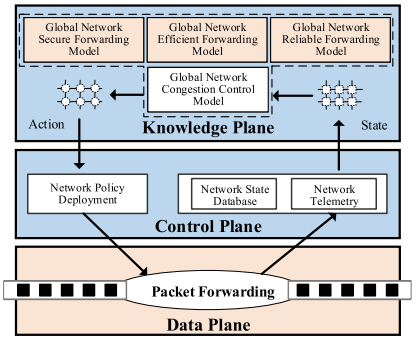
\includegraphics[width=\textwidth]{figures/fig2.png}

      \vspace{0.15cm}
      \begin{tcolorbox}[
        enhanced, boxrule=0pt,
        colback=white, colframe=white,
        arc=4pt, left=6pt, right=6pt,
        top=3pt, bottom=3pt,
        borderline west={4pt}{0pt}{problemorange},
      ]
        \scriptsize\textcolor{problemorange}{\bfseries AI in Controller:}
        \textcolor{HUAdark}{High inter-plane latency ---
        coarse-grained telemetry only.}
      \end{tcolorbox}
    \end{column}

    % ── Vertical Divider ─────────────────────────────────
    \begin{column}{0.02\textwidth}
      \centering
      \textcolor{HUAlight}{\rule{0.5pt}{0.75\textheight}}
    \end{column}

    % ── Right: Programmable Data Plane (Fig. 3) ───────────
    \begin{column}{0.400\textwidth}
      \centering

      {\color{HUAdark}\bfseries\small Programmable Data Plane — Framework II}
      \vspace{0.15cm}

      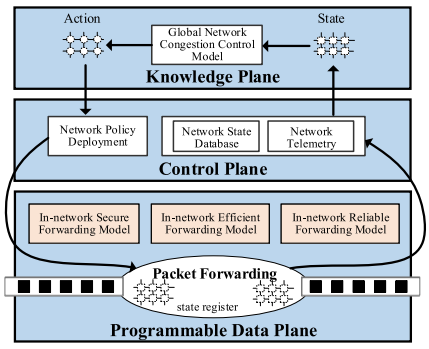
\includegraphics[width=\textwidth]{figures/fig3.png}

      \vspace{0.15cm}
      \begin{tcolorbox}[
        enhanced, boxrule=0pt,
        colback=white, colframe=white,
        arc=4pt, left=6pt, right=6pt,
        top=3pt, bottom=3pt,
        borderline west={4pt}{0pt}{solutiongreen},
      ]
        \scriptsize\textcolor{solutiongreen}{\bfseries AI inside Switch:}
        \textcolor{HUAdark}{Wire-speed decisions ---
        fine-grained telemetry available.}
      \end{tcolorbox}
    \end{column}

  \end{columns}

\end{frame}
}
{
\metroset{titleformat frame=smallcaps}
\begin{frame}{The P4 Programming Language}

  \subtitlebar{The tool that translates AI decisions into hardware actions}

  \vspace{0.10cm}

  \begin{center}
    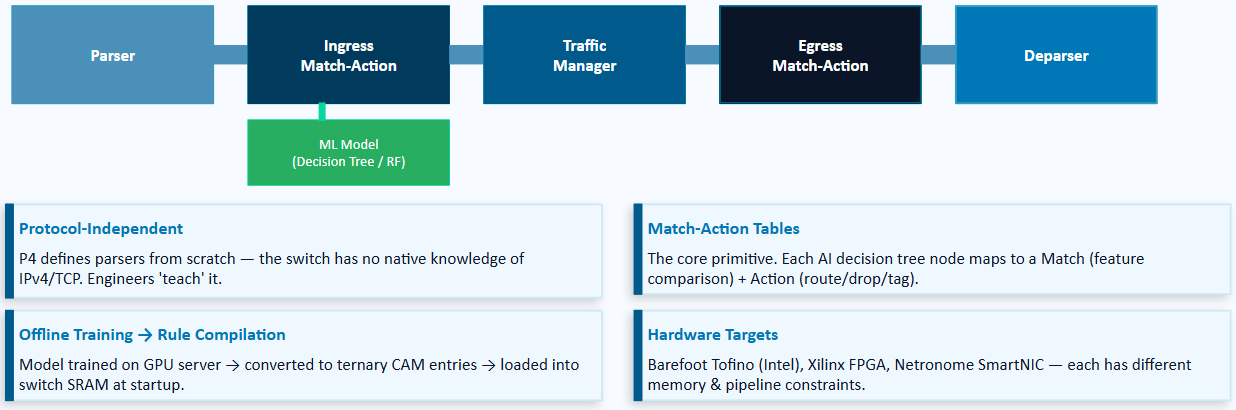
\includegraphics[width=1.0\textwidth, 
                     height=0.82\textheight, 
                     keepaspectratio]{figures/p4.png}
  \end{center}

\end{frame}
}





   % Background: PDP & P4
\section{AI Integration in the Data Plane}

{
\metroset{titleformat frame=smallcaps}
\begin{frame}{AI Integration Workflow \& Hardware Constraints}

  \subtitlebar{From training on a GPU server to wire-speed inference inside a switch}

  \begin{columns}[T, totalwidth=\textwidth]

    % ── Left: Workflow ────────────────────────────────────
    \begin{column}{0.488\textwidth}
      {\color{HUAblue}\bfseries\small The Integration Workflow}
      \vspace{6pt}
      \begin{itemize}
        \setlength\itemsep{8pt}
        \footnotesize
        \item[\textcolor{HUAblue}{\bfseries 1}]
          \textbf{Data Collection} ---
          INT probes collect fine-grained
          per-packet features (queue depth,
          inter-arrival time, 5-tuple).
        \item[\textcolor{HUAblue}{\bfseries 2}]
          \textbf{Offline Training} ---
          Lightweight models (DT, RF, SVM)
          trained on external server
          with labeled dataset.
        \item[\textcolor{HUAblue}{\bfseries 3}]
          \textbf{Model Compression} ---
          Pruning \& quantization reduce
          floating-point ops. Depth $\leq$ 5,
          features $\leq$ 15 for SRAM fit.
        \item[\textcolor{HUAblue}{\bfseries 4}]
          \textbf{Rule Translation} ---
          Model converted to TCAM
          Match-Action entries
          (pForest, IIsy, Planter).
        \item[\textcolor{HUAblue}{\bfseries 5}]
          \textbf{P4 Deployment} ---
          Rules loaded into switch pipeline.
          Inference at line-rate
          ($\sim$hundreds of ns).
      \end{itemize}
    \end{column}

    % ── Vertical Divider ─────────────────────────────────
    \begin{column}{0.02\textwidth}
      \textcolor{HUAlight}{\rule{0.5pt}{0.55\textheight}}
    \end{column}

    % ── Right: Hardware Constraints ───────────────────────
    \begin{column}{0.468\textwidth}
      {\color{problemorange}\bfseries\small Key Hardware Constraints}
      \vspace{6pt}
      \begin{itemize}
        \setlength\itemsep{8pt}
        \footnotesize
        \item[\textcolor{problemorange}{\bfseries C1}]
          \textbf{No Floating Point} ---
          ASICs use integer arithmetic only.
          All weights must be quantized
          before deployment.
        \item[\textcolor{problemorange}{\bfseries C2}]
          \textbf{SRAM $\approx$ 10--40~MB} ---
          Shared with forwarding tables.
          Decision trees limited to
          depth 5--10, $\leq$ 256 leaves.
        \item[\textcolor{problemorange}{\bfseries C3}]
          \textbf{Stateless Stages} ---
          P4 stages are largely stateless.
          Recurrent models (LSTM) cannot
          run natively.
        \item[\textcolor{problemorange}{\bfseries C4}]
          \textbf{Pipeline Width} ---
          Tofino has $\sim$12 ingress stages.
          Complex DNNs with 100+ ops
          are infeasible.
      \end{itemize}
    \end{column}

  \end{columns}

\end{frame}
}
{
\metroset{titleformat frame=smallcaps}
\begin{frame}{Network Delay Components \& PDP}

  \subtitlebar{Where exactly does the PDP intervene
               in each delay component}

  \begin{center}
    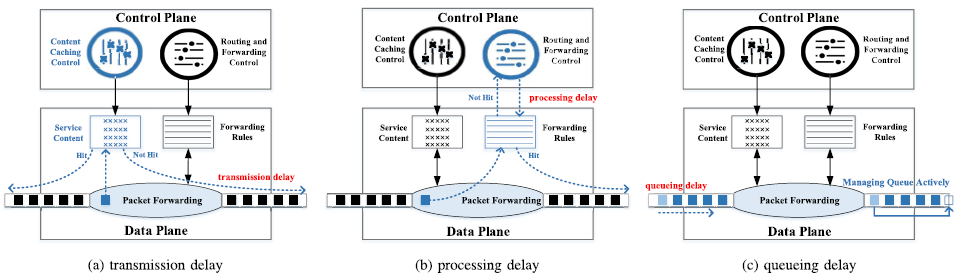
\includegraphics[width=0.92\textwidth,
                     height=0.80\textheight,
                     keepaspectratio]{figures/fig4.png}
  \end{center}

  \begin{center}
    {\scriptsize\itshape\color{HUAdark}
      Three Network Delay Components and Corresponding
      Switch Operating Position ---
      The Blue Part}
  \end{center}

\end{frame}
}
{
\metroset{titleformat frame=smallcaps}
\begin{frame}{How PDP Addresses Each Delay Type}

  \subtitlebar{AI and PDP reduce delay at every stage of the forwarding pipeline}

  \begin{columns}[T, totalwidth=\textwidth]

    % ── Transmission Delay ────────────────────────────────
    \begin{column}{0.31\textwidth}
      \begin{tcolorbox}[problemcard=HUAblue]
        {\color{HUAblue}\bfseries\small
          Transmission Delay}
        \vspace{4pt}
        \begin{itemize}
          \setlength\itemsep{3pt}
          \fontsize{7}{8}\selectfont\color{HUAdark}
          \item Depends on distance between
                user and data provider.
          \item AI predicts content popularity
                and caches it at nearby nodes.
          \item PDP collects accurate link-state
                to select the shortest path.
        \end{itemize}
      \end{tcolorbox}
    \end{column}

    % ── Processing Delay ──────────────────────────────────
    \begin{column}{0.31\textwidth}
      \begin{tcolorbox}[problemcard=problemorange]
        {\color{problemorange}\bfseries\small
          Processing Delay}
        \vspace{4pt}
        \begin{itemize}
          \setlength\itemsep{3pt}
          \fontsize{7}{8}\selectfont\color{HUAdark}
          \item Caused by forwarding rule
                lookup and controller
                communication overhead.
          \item RL model manages rule
                placement between switch
                and controller.
          \item PDP caches rules locally ---
                reducing controller round-trips.
        \end{itemize}
      \end{tcolorbox}
    \end{column}

    % ── Queueing Delay ────────────────────────────────────
    \begin{column}{0.31\textwidth}
      \begin{tcolorbox}[problemcard=solutiongreen]
        {\color{solutiongreen}\bfseries\small
          Queueing Delay}
        \vspace{4pt}
        \begin{itemize}
          \setlength\itemsep{3pt}
          \fontsize{7}{8}\selectfont\color{HUAdark}
          \item Caused by packet congestion
                in switch queues.
          \item AQM algorithms (PI2, CoDel)
                deployed directly on P4
                switches.
          \item AI classifies flows and
                assigns priority queues
                in real time.
        \end{itemize}
      \end{tcolorbox}
    \end{column}

  \end{columns}

\end{frame}
}
   % AI Integration in the Data Plane
\section{Taxonomy of AI-Driven Forwarding}

{
\metroset{titleformat frame=smallcaps}
\begin{frame}{Taxonomy of AI-Driven Forwarding}

  \subtitlebar{Four performance dimensions improved by AI and PDP}

  \begin{columns}[T, totalwidth=\textwidth]

    % ── Left column ───────────────────────────────────────
    \begin{column}{0.488\textwidth}

      % Card 1 — Delay
      \begin{tcolorbox}[problemcard=HUAblue]
        {\color{HUAblue}\bfseries\small
          I. Delay Reduction}
        \vspace{4pt}
        \begin{itemize}
          \setlength\itemsep{2pt}
          \footnotesize
          \item AI models proactively manage queues
                to achieve sub-millisecond latency.
          \item AQM algorithms (PI2, CoDel) deployed
                directly on P4 switches.
          \item Moving from static to dynamic,
                traffic-aware forwarding.
        \end{itemize}
      \end{tcolorbox}

      \vspace{8pt}

      % Card 3 — Security
      \begin{tcolorbox}[problemcard=problemred]
        {\color{problemred}\bfseries\small
          III. Security}
        \vspace{4pt}
        \begin{itemize}
          \setlength\itemsep{2pt}
          \footnotesize
          \item Lightweight ML (Random Forests)
                detects and drops DDoS and
                ransomware packets at wire-speed.
          \item Threats handled at switch level ---
                before reaching the controller.
          \item In-network models: pForest,
                SwitchTree, ML-Pushback.
        \end{itemize}
      \end{tcolorbox}

    \end{column}

    % ── Right column ──────────────────────────────────────
    \begin{column}{0.488\textwidth}

      % Card 2 — Throughput
      \begin{tcolorbox}[problemcard=HUAlight]
        {\color{HUAlight}\bfseries\small
          II. Throughput Enhancement}
        \vspace{4pt}
        \begin{itemize}
          \setlength\itemsep{2pt}
          \footnotesize
          \item Intelligent multi-path routing
                dynamically avoids congested links.
          \item RL-based congestion control
                (SmartCC, TCP-PPCC) maximizes
                available bandwidth.
          \item PDP telemetry provides accurate
                link-state (HULA, PINT).
        \end{itemize}
      \end{tcolorbox}

      \vspace{8pt}

      % Card 4 — Reliability
      \begin{tcolorbox}[problemcard=solutiongreen]
        {\color{solutiongreen}\bfseries\small
          IV. Reliability}
        \vspace{4pt}
        \begin{itemize}
          \setlength\itemsep{2pt}
          \footnotesize
          \item INT / P-INT telemetry with
                minimal overhead extension.
          \item RL congestion avoidance detects
                failures before they occur.
          \item Runtime P4 verification ensures
                the network behaves as intended.\newline
        \end{itemize}
      \end{tcolorbox}

    \end{column}

  \end{columns}

\end{frame}
}   % Taxonomy of AI-Driven Forwarding
\section{Key Use Cases \& Applications}

{
\metroset{titleformat frame=smallcaps}
\begin{frame}{Use Case 1: Smart Congestion Control}
\vspace{6pt}
  \subtitlebar{Reinforcement Learning + INT telemetry for proactive traffic management}

  \begin{columns}[T, totalwidth=\textwidth]

    % ── Left: 3 Boxes ─────────────────────────────────────
    \begin{column}{0.44\textwidth}

      \begin{tcolorbox}[problemcard=problemred]
        {\color{problemred}\bfseries\scriptsize The Problem}\\[2pt]
        {\footnotesize\color{HUAdark}
          Traditional networks rely on static paths,
          causing bottlenecks during sudden traffic
          bursts (\textit{Elephant Flows}).}
      \end{tcolorbox}

      \vspace{4pt}

      \begin{tcolorbox}[problemcard=HUAblue]
        {\color{HUAblue}\bfseries\scriptsize AI in Action}\\[2pt]
        {\footnotesize\color{HUAdark}
          A Reinforcement Learning model monitors
          link and node load via INT telemetry,
          and adjusts routing rules in real time.}
      \end{tcolorbox}

      \vspace{4pt}

      \begin{tcolorbox}[problemcard=solutiongreen]
        {\color{solutiongreen}\bfseries\scriptsize Result}\\[2pt]
        {\footnotesize\color{HUAdark}
          Optimal routing rules applied at wire-speed ---
          maximizing bandwidth and preventing
          congestion proactively.}
      \end{tcolorbox}

    \end{column}

    % ── Vertical Divider ─────────────────────────────────
    \begin{column}{0.02\textwidth}
      \centering
      \textcolor{HUAlight}{\rule{0.5pt}{0.80\textheight}}
    \end{column}

    % ── Right: Fig. 10 ───────────────────────────────────
    \begin{column}{0.45\textwidth}
      \centering
      \vspace{0.15cm}
      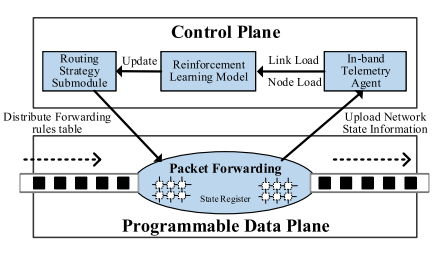
\includegraphics[width=\textwidth]{figures/fig10.png}
      \vspace{0.15cm}
      \begin{tcolorbox}[
        enhanced, boxrule=0pt,
        colback=HUApale, colframe=HUApale,
        arc=3pt, left=5pt, right=5pt,
        top=2pt, bottom=2pt,
      ]
        \centering
        \scriptsize\color{HUAdark}\itshape
        Framework of Network Congestion Control
        %(Quan et al., Fig.~10)
      \end{tcolorbox}
    \end{column}

  \end{columns}

\end{frame}
}
{
\metroset{titleformat frame=smallcaps}
\begin{frame}{Use Case 2: Wire-Speed DDoS Defense}
\vspace{6pt}
  \subtitlebar{Lightweight ML at the data plane eliminates controller-based reaction lag}

  \begin{columns}[T, totalwidth=\textwidth]

    % ── Left: 3 Boxes ─────────────────────────────────────
    \begin{column}{0.44\textwidth}

      \begin{tcolorbox}[problemcard=problemred]
        {\color{problemred}\bfseries\scriptsize The Threat}\\[2pt]
        {\footnotesize\color{HUAdark}
          DDoS attacks flood the network with
          massive traffic, aiming to overwhelm
          and paralyze the central controller.}
      \end{tcolorbox}

      \vspace{6pt}

      \begin{tcolorbox}[problemcard=HUAblue]
        {\color{HUAblue}\bfseries\scriptsize AI in Action}\\[2pt]
        {\footnotesize\color{HUAdark}
          Lightweight ML models analyze packet
          features locally (IP, UDP, TCP, SYN
          counts) and classify traffic in real time.}
      \end{tcolorbox}

      \vspace{6pt}

      \begin{tcolorbox}[problemcard=solutiongreen]
        {\color{solutiongreen}\bfseries\scriptsize PDP Result}\\[2pt]
        {\footnotesize\color{HUAdark}
          Malicious packets are dropped directly
          at the switch --- no controller round-trip,
          no attack reaches the server.}
      \end{tcolorbox}

    \end{column}

    % ── Vertical Divider ─────────────────────────────────
    \begin{column}{0.02\textwidth}
      \centering
      \textcolor{HUAlight}{\rule{0.5pt}{0.83\textheight}}
    \end{column}

    % ── Right: Fig. 6 ────────────────────────────────────
    \begin{column}{0.45\textwidth}
      \centering
      \vspace{0.15cm}
      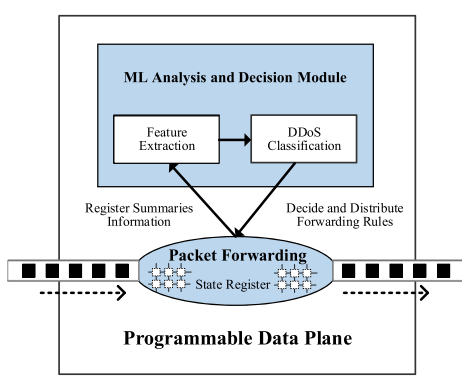
\includegraphics[width=\textwidth]{figures/fig6.png}
      \vspace{0.15cm}
      \begin{tcolorbox}[
        enhanced, boxrule=0pt,
        colback=HUApale, colframe=HUApale,
        arc=3pt, left=5pt, right=5pt,
        top=2pt, bottom=2pt,
      ]
        \centering
        \scriptsize\color{HUAdark}\itshape
        Defending DDoS Attacks with AI and PDP
        %(Quan et al., Fig.~6)
      \end{tcolorbox}
    \end{column}

  \end{columns}

\end{frame}
}
{
\metroset{titleformat frame=smallcaps}
\begin{frame}{Use Case 3: Ransomware Detection at the Network Edge}
      \vspace{7pt}
  \subtitlebar{Moving defense from the user device to the switch --- before the attack arrives}

  \begin{columns}[T, totalwidth=\textwidth]

    % ── Left: 3 Boxes ─────────────────────────────────────
    \begin{column}{0.44\textwidth}

      \begin{tcolorbox}[problemcard=problemred]
        {\color{problemred}\bfseries\scriptsize The Threat}\\[2pt]
        {\footnotesize\color{HUAdark}
        Ransomware hijacks files and extorts money.
        Traditional defenses activate only after
        the attack reaches the device.}
      \end{tcolorbox}

      \vspace{6pt}

      \begin{tcolorbox}[problemcard=HUAblue]
        {\color{HUAblue}\bfseries\scriptsize AI in Action}\\[2pt]
        {\footnotesize\color{HUAdark}
          PDP collects 5-tuple, timestamp and byte count.
          A Random Forest (40 trees, depth 15)
          classifies each stream in real time.}
      \end{tcolorbox}

      \vspace{6pt}

      \begin{tcolorbox}[problemcard=solutiongreen]
        {\color{solutiongreen}\bfseries\scriptsize PDP Result}\\[2pt]
        {\footnotesize\color{HUAdark}
          Attack traffic intercepted at the
          switch --- before reaching the user.
          Detection accuracy: \textbf{86\%},
          failure rate: only \textbf{11\%}.}
      \end{tcolorbox}

    \end{column}

    % ── Vertical Divider ─────────────────────────────────
    \begin{column}{0.02\textwidth}
      \centering
      \textcolor{HUAlight}{\rule{0.5pt}{0.80\textheight}}
    \end{column}

    % ── Right: Fig. 7 ────────────────────────────────────
    \begin{column}{0.45\textwidth}
      \centering
      \vspace{0.15cm}
      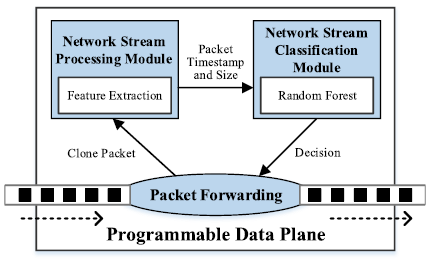
\includegraphics[width=\textwidth]{figures/fig7.png}
      \vspace{0.15cm}
      \begin{tcolorbox}[
        enhanced, boxrule=0pt,
        colback=HUApale, colframe=HUApale,
        arc=3pt, left=5pt, right=5pt,
        top=2pt, bottom=2pt,
      ]
        \centering
        \scriptsize\color{HUAdark}\itshape
        Mechanism on Defending Ransomware Attack
        with ML and PDP
      \end{tcolorbox}
    \end{column}

  \end{columns}

\end{frame}
}   % Key Use Cases & Applications
\section{Open Challenges \& Limitations}


{
\metroset{titleformat frame=smallcaps}
\begin{frame}{Open Challenges \& Limitations}
\vspace{4pt}
  \subtitlebar{Key barriers before autonomous in-network AI can be deployed at scale}

  % ── 6 Boxes in 2x3 Grid ──────────────────────────────────
  \begin{columns}[T, totalwidth=\textwidth]

    % ── Left Column ───────────────────────────────────────
    \begin{column}{0.488\textwidth}

      \begin{tcolorbox}[problemcard=problemorange]
        {\color{problemorange}\bfseries\scriptsize
          C1 — SRAM Limits}\\[2pt]
        {\fontsize{7}{8}\selectfont\color{HUAdark}
          Switch SRAM is shared with forwarding tables.
          Decision trees limited to depth 5--10 in practice.}
      \end{tcolorbox}

      \vspace{4pt}

      \begin{tcolorbox}[problemcard=problemorange]
        {\color{problemorange}\bfseries\scriptsize
          C2 — Translation Gap}\\[2pt]
        {\fontsize{7}{8}\selectfont\color{HUAdark}
          Converting ML models into P4 Match-Action
          rules without losing accuracy remains difficult.}
      \end{tcolorbox}

      \vspace{4pt}

      \begin{tcolorbox}[problemcard=problemorange]
        {\color{problemorange}\bfseries\scriptsize
          C3 — Resource Trade-offs}\\[2pt]
        {\fontsize{7}{8}\selectfont\color{HUAdark}
          Memory allocated to AI models reduces space
          for basic functions like routing tables.}
      \end{tcolorbox}

    \end{column}

    % ── Right Column ──────────────────────────────────────
    \begin{column}{0.488\textwidth}

      \begin{tcolorbox}[problemcard=problemred]
        {\color{problemred}\bfseries\scriptsize
          C4 — Dataset Scarcity}\\[2pt]
        {\fontsize{7}{8}\selectfont\color{HUAdark}
          High-quality labeled network traffic datasets
          are rare. Synthetic datasets may not reflect
          real topologies.}
      \end{tcolorbox}

      \vspace{4pt}

      \begin{tcolorbox}[problemcard=problemred]
        {\color{problemred}\bfseries\scriptsize
          C5 — Adversarial ML}\\[2pt]
        {\fontsize{7}{8}\selectfont\color{HUAdark}
          Attackers can craft packets to fool in-network
          classifiers. Models inside switches are
          harder to retrain.}
      \end{tcolorbox}

      \vspace{4pt}

      \begin{tcolorbox}[problemcard=problemred]
        {\color{problemred}\bfseries\scriptsize
          C6 — No Standardization}\\[2pt]
        {\fontsize{7}{8}\selectfont\color{HUAdark}
          Tofino, FPGA, SmartNIC use different P4
          architectures --- no universal cross-platform
          toolchain exists.}
      \end{tcolorbox}

    \end{column}

  \end{columns}

  \vspace{0.15cm}

% ── Legend — one line ─────────────────────────────────────
\begin{columns}[totalwidth=\textwidth]
  \begin{column}{0.488\textwidth}
    {\fontsize{7}{8}\selectfont
      \textcolor{problemorange}{\rule{0.8em}{0.8em}}~
      \textcolor{problemorange}{\bfseries Technical}
      --- hardware constraints inside the switch}
  \end{column}
  \begin{column}{0.488\textwidth}
    {\fontsize{7}{8}\selectfont
      \textcolor{problemred}{\rule{0.8em}{0.8em}}~
      \textcolor{problemred}{\bfseries Deployment}
      --- practical barriers outside the switch}
  \end{column}
\end{columns}

\end{frame}
}   % Open Challenges & Limitations
\section{Future Directions \& Conclusion}

{
\metroset{titleformat frame=smallcaps}
\begin{frame}{AI-Driven Forwarding: Future Landscape}
 \vspace{6pt}
  \subtitlebar{Future trends, challenges and open issues of AI-driven packet forwarding}

  \begin{center}
    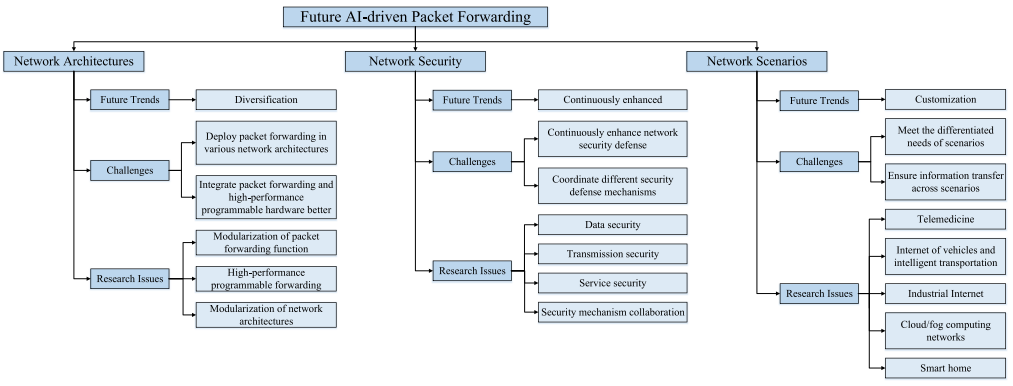
\includegraphics[width=1.0\textwidth,
                     height=0.80\textheight,
                     keepaspectratio]{figures/fig12.png}
  \end{center}

  \vspace{0.05cm}

  \begin{center}
    {\scriptsize\itshape\color{HUAdark}
      Future Trends and Open Issues of AI-driven
      Packet Forwarding}
  \end{center}

\end{frame}
}
{
\metroset{titleformat frame=smallcaps}
\begin{frame}{Future Directions: The Road Ahead}

  \subtitlebar{Three convergence vectors identified by the survey}

  \begin{columns}[T, totalwidth=\textwidth]

    % ── Direction 1 ───────────────────────────────────────
    \begin{column}{0.31\textwidth}
      \begin{tcolorbox}[problemcard=HUAblue]
        {\color{HUAblue}\bfseries\small
          Direction 1}\\[2pt]
        {\color{HUAblue}\bfseries\scriptsize
          Network Architectures}
        \vspace{4pt}
        \begin{itemize}
          \setlength\itemsep{3pt}
          \fontsize{7}{8}\selectfont\color{HUAdark}
          \item Moving towards high-performance
                modular programmable hardware.
          \item Integration with 6G networks
                and new forwarding paradigms.
          \item Modularization of packet
                forwarding functions.\newline
        \end{itemize}
      \end{tcolorbox}
    \end{column}

    % ── Direction 2 ───────────────────────────────────────
    \begin{column}{0.31\textwidth}
      \begin{tcolorbox}[problemcard=problemorange]
        {\color{problemorange}\bfseries\small
          Direction 2}\\[2pt]
        {\color{problemorange}\bfseries\scriptsize
          Enhanced Network Security}
        \vspace{4pt}
        \begin{itemize}
          \setlength\itemsep{3pt}
          \fontsize{7}{8}\selectfont\color{HUAdark}
          \item Collaborative defense mechanisms
                protecting both network and
                AI models.
          \item Coordination across IDS, IPS,
                firewall and audit systems.
          \item Blockchain integration for
                decentralized packet audit.
        \end{itemize}
      \end{tcolorbox}
    \end{column}

    % ── Direction 3 ───────────────────────────────────────
    \begin{column}{0.31\textwidth}
      \begin{tcolorbox}[problemcard=solutiongreen]
        {\color{solutiongreen}\bfseries\small
          Direction 3}\\[2pt]
        {\color{solutiongreen}\bfseries\scriptsize
          Customized Network Scenarios}
        \vspace{4pt}
        \begin{itemize}
          \setlength\itemsep{3pt}
          \fontsize{7}{8}\selectfont\color{HUAdark}
          \item Telemedicine: sub-ms latency
                for remote surgery networks.
          \item Industrial Internet and
                Internet of Vehicles.
          \item Smart Home and IoT with
                lightweight on-device AI. \newline \newline
        \end{itemize}
      \end{tcolorbox}
    \end{column}

  \end{columns}

\end{frame}
}
{
\metroset{titleformat frame=smallcaps}
\begin{frame}{Conclusion: A New Era for Networking}
  \vspace{6pt}
  \subtitlebar{From centralized SDN intelligence to distributed wire-speed AI}

  \begin{tcolorbox}[problemcard=HUAdark]
    {\color{HUAdark}\bfseries\small The Paradigm Shift}
    \vspace{3pt}\\
    {\footnotesize\color{HUAdark}
      We are transitioning from \textbf{centralized SDN control}
      to \textbf{localized, wire-speed in-network AI} ---
      powered by Programmable Data Planes and P4.}
  \end{tcolorbox}

  \vspace{6pt}

  \begin{tcolorbox}[problemcard=HUAdark]
    {\color{HUAdark}\bfseries\small The Power of P4}
    \vspace{3pt}\\
    {\footnotesize\color{HUAdark}
      Programmable Data Planes \textbf{break the limits}
      of traditional fixed-function switches ---
      enabling AI to run directly inside the switch fabric
      at wire-speed.}
  \end{tcolorbox}

  \vspace{6pt}

  \begin{tcolorbox}[problemcard=HUAdark]
    {\color{HUAdark}\bfseries\small The Ultimate Vision}
    \vspace{3pt}\\
    {\footnotesize\color{HUAdark}
      Truly \textbf{autonomous networks} capable of
      wire-speed self-optimization, self-healing and
      self-defense --- the foundation for 6G and beyond.}
  \end{tcolorbox}

  \vspace{8pt}

% ── Final Takeaway ────────────────────────────────────────
  \begin{tcolorbox}[
    enhanced, boxrule=0pt,
    colback=HUApale, colframe=HUApale,
    arc=4pt, left=8pt, right=8pt,
    top=4pt, bottom=4pt,
    borderline west={4pt}{0pt}{HUAblue},
  ]
    \centering\footnotesize\color{HUAdark}
    \textbf{AI + PDP} improves all four dimensions ---
    \textcolor{HUAblue}{\bfseries Delay},
    \textcolor{HUAlight}{\bfseries Throughput},
    \textcolor{problemred}{\bfseries Security} and
    \textcolor{solutiongreen}{\bfseries Reliability} ---
    bringing us closer to fully autonomous networks.\\[4pt]
    In our view, the key open challenge remains the
    \textbf{translation gap} --- converting ML models
    into P4 rules without accuracy loss.
  \end{tcolorbox}

\end{frame}
}


   % Future Directions
% ── Repository ───────────────────────────────────────────
{
\setbeamertemplate{frame footer}{}
\setbeamertemplate{frame numbering}{}
\begin{frame}{Project Repository}
  \begin{center}

    Get the full \LaTeX\ source of this presentation from\\[8pt]

    {\color{HUAblue}\bfseries
      \href{https://github.com/drososkats/ai-driven-packet-forwarding-pdp}
           {github.com/drososkats/ai-driven-packet-forwarding-pdp}}

    \vspace{8pt}

    \ccbysa

    \vspace{8pt}

    {\footnotesize
      Katsimpras Drosos (ais25123)\\
      Harokopio University of Athens\\
      Academic Year 2025--2026}

  \end{center}
\end{frame}
}

{\setbeamercolor{palette primary}{fg=black, bg=HUAblue}
\begin{frame}[standout, plain]
    \textcolor{white}{\textbf{Thank you! / Questions?}}
   ~\alert{\faSmile}~
\end{frame}
}

\appendix
\setbeamertemplate{frame footer}{}
\begin{frame}{List of Abbreviations}
 
  \subtitlebar{Key terms and acronyms used throughout this presentation}
 
  \begin{columns}[T, totalwidth=\textwidth]
 
    \begin{column}{0.488\textwidth}
      \begin{tcolorbox}[problemcard=HUAblue]
        \begin{tabular}{@{} l @{\hspace{8pt}} l @{}}
          \abbr{AI}   {Artificial Intelligence}
          \abbr{AQM}  {Active Queue Management}
          \abbr{DDoS} {Distributed Denial of Service}
          \abbr{INT}  {In-band Network Telemetry}
          \abbr{IoT}  {Internet of Things}
          \abbr{ML}   {Machine Learning}
        \end{tabular}
      \end{tcolorbox}
    \end{column}
 
    \begin{column}{0.488\textwidth}
      \begin{tcolorbox}[problemcard=HUAblue]
        \begin{tabular}{@{} l @{\hspace{8pt}} l @{}}
          \abbr{PDP}   {Programmable Data Plane}
          \abbr{RF}    {Random Forest}
          \abbr{SDN}   {Software Defined Network}
          \abbr{SRAM}  {Static Random Access Memory}
          \abbr{TCAM}  {Ternary Content Addressable Mem.}
          \abbr{URLLC} {Ultra-Reliable Low-Latency Comm.}
        \end{tabular}
      \end{tcolorbox}
    \end{column}

  \end{columns}

\end{frame}

% ── References ───────────────────────────────
\begin{frame}[allowframebreaks]{References}
\nocite{*}
  \bibliographystyle{plain}
  \bibliography{references}
\end{frame}    % Conclusion

% ============================================================
\end{document}